\documentclass[10pt, conference, compsocconf]{IEEEtran}

%% Custom TeX

\usepackage{listings}
\usepackage{xspace}
\usepackage{graphicx}
\usepackage{caption}
\usepackage{subcaption}
\usepackage{rotating}
\usepackage{geometry}
\usepackage{amssymb}
\usepackage{url}
\usepackage[splitrule]{footmisc}

\usepackage[dvipsnames]{xcolor}

\usepackage{listings}
\lstloadlanguages{Ruby,Java}
\lstset{
basicstyle=\ttfamily\color{black},
commentstyle = \ttfamily\color{red},
keywordstyle=\ttfamily\color{blue},
stringstyle=\color{orange}}

%% for comments
\newcommand{\comment}[3][\color{red}]{{#1{[{#2}: {#3}]}}}
\newcommand{\code}[1]{\textsf{\small #1}}
\newcommand{\kris}[1]{\comment[\color{orange}]{km}{#1}}

\newcommand{\thickhline}{\noalign{\hrule height 1pt}}

%% End of custom TeX

\begin{document}
%
% --- Author Metadata here ---
% --- End of Author Metadata ---

\title{MapReduce to My Ears\\
{\Large Using Big Data for Music Synthesis}
}

%%\numberofauthors{3}
\author{
\IEEEauthorblockN{Christopher Imbriano, Amanda Strickler, Kristopher Micinski}
\IEEEauthorblockA{Computer Science Department, University of Maryland,
  College Park, MD 20742, USA
}
}

\maketitle

\begin{abstract}
Every young computer scientist learns early in their career that all
data regardless of its meaning are all the same in their underlying
representation - simple ones and zeroes.
 It is only in the act of
reading and subsequently interpreting those data that computer
scientists or their creations give meaning to the bits and bytes.
MapReduce to My Ears is an exercise in the reinterpretation of data
meant to be understood as color and picture into sound and music.
Our method uses Hadoop, an open source implementation of the MapReduce
programming paradigm, to process a large corpus of images and extract
a musical representation.
 We have produce a six minutes and
thirty-five second audio/visual entitled \emph{Digital Nightmare}, the
style of which can be described as 8-bit, blast beat.
\end{abstract}

\section{Introduction}
\label{sec:introduction}

Big data has revolutionized the way we think about, design, and
implement algorithms at scale.  As such, problems from all different
areas of computer science have been lifted into the MapReduce
framework.  While MapReduce has been applied to many large-scale data
processing domains, it has been used relatively less to explore art or
creative tasks.  Our project looks to answer: what kinds of art can we
create harnessing large amounts of data at scale?

We present a system to synthesize music using large amounts of data.
The input is a large corpus of images, which is subsequently processed
by our system, and the result is a musical score.  We then mix,
listen, and refine the algorithm to produce art.

\subsection{Motivation} 

We are currently unaware of any projects using MapReduce to create art
or any other representation of digital media.  Because of this, we
anticipate that there might be problems in handling media (buffering,
representing, etc..).  We anticipate that exploring this area might
open up potential applications.

\section{Overview}
\label{sec:overview}

The core idea in converting image data to music is to view the
information in an image (color, size, opacity, etc..) as a mapping to
notes and durations with which those notes are sustained.  In our
system we chose MIDI as the output format.  Our system can then be
modeled as a function from image data to MIDI output.  Using MIDI as a
format works well because it is easy to work with (we can model music
as MIDI events, which are simply streams of musical data) and can be
mixed by many synthesizers to produce music using a variety of
instruments.

Our system takes in ordered sets of images and produces a MIDI file.
The input format is JPEG images: this is a very commonly used lossy
compression format.  Since we used input corpuses from the internet,
using JPEG worked for the variety of input formats.  Using JPEG as the
input format is also attractive because it can be easily unpacked by
the Java \code{ImageBuffer} class.  

The output of our MapReduce phases is MIDI music.  MIDI is a simple
format for writing music which can be mixed ans synthesized using
software.  At an abstract level, a MIDI file consists of note and
duration pairs.  Taken together, these constitute a score by chaining
together multiple pairs over the course of time:

\[
MIDI : (Note,Duration)^{\ast}
\]

However, producing a MIDI score with only a single instrument would
sound broing (akin to a song with only one player): instead we take
pieces of images and map them into different parts.  Each of these
parts constitutes an instrument and --- when mixed together ---
produces a final score.  An illustration of the core idea is shown in
Figure~\ref{fig:images-to-music}.

\begin{figure*}
  \centering
  \begin{minipage}[t]{.3\textwidth}
    \centering
    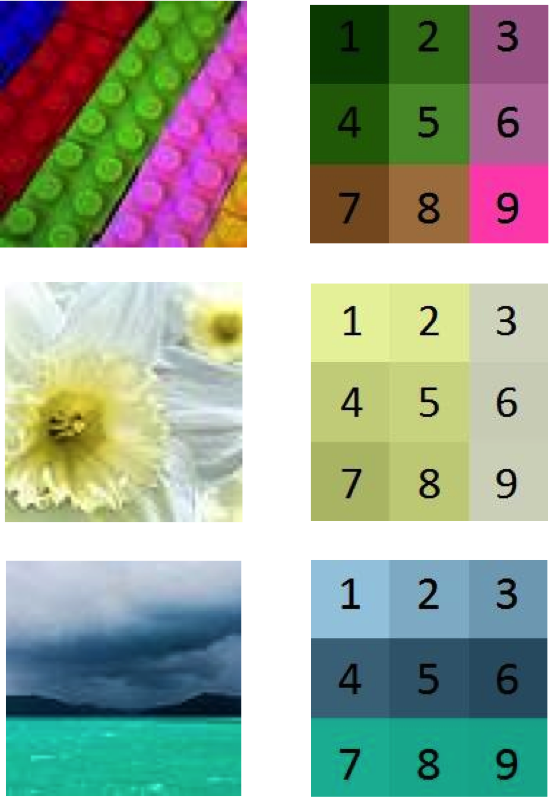
\includegraphics[width=.7\textwidth]{images-to-regions.png}
  \end{minipage}
  \begin{minipage}[t]{.1\textwidth}
    \raisebox{.8 in}{\Huge $\to$}
  \end{minipage}
  \begin{minipage}[t]{.4\textwidth}
    \centering
    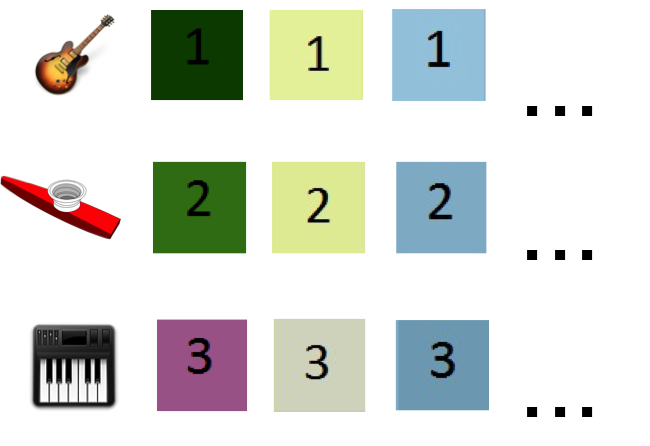
\includegraphics[width=\textwidth]{parts-and-instruments.png}
  \end{minipage}
  \caption{Mapping a stream of three images to a nine piece musical
    score.  First each image is mapped into regions, which will be
    transformed into notes and combined into a score using a mixer.}
\end{figure*}
  
\begin{figure}
  \centering
  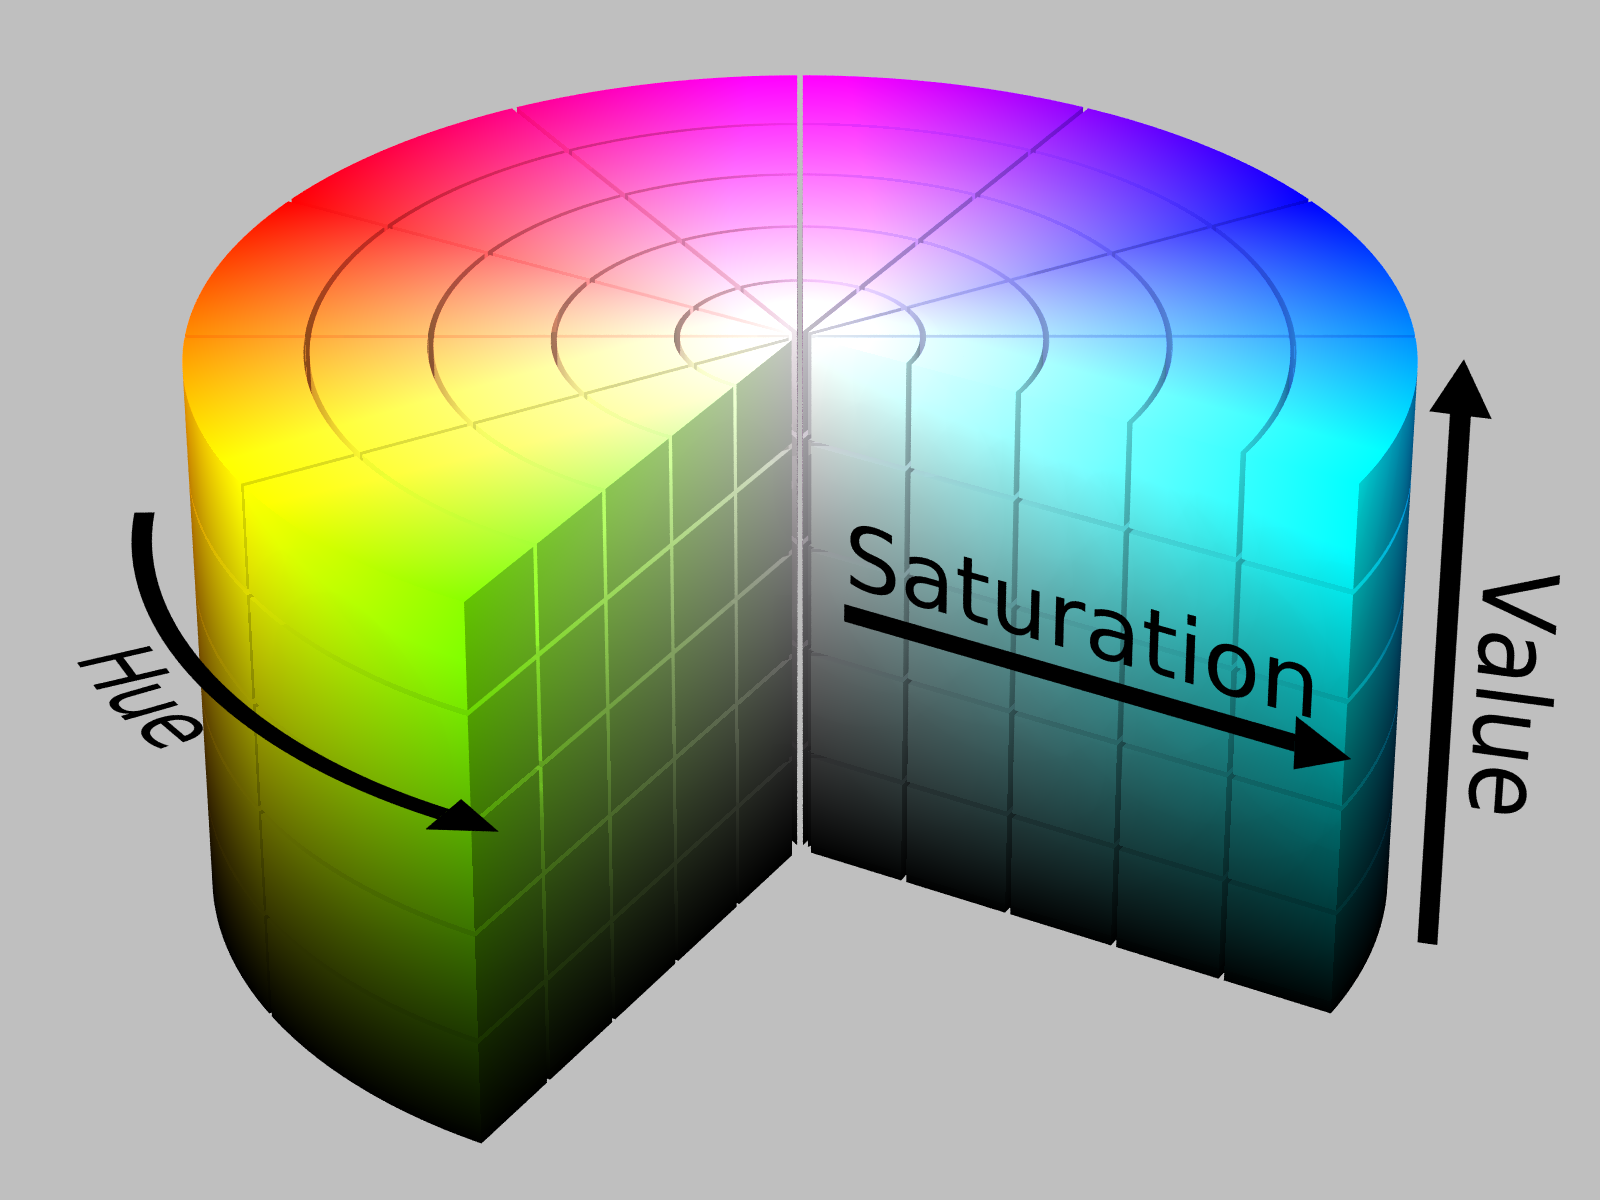
\includegraphics[width=.4\textwidth]{hsv.png}
  \caption{The HSV color cylinder}
  \label{fig:hsv}
\end{figure}

\subsection{The HSV format}

To convert image data to musical notes, we need to establish a
bijection between the data in the image and the range of music in the
song.  The way we do this is inspired by viewing colors in images as
HSV values.  In HSV, each color has three components: a hue, a
saturation, and a value.  These components are visualized (as shown in
Figure~\ref{fig:hsv}) as a cylinder (as opposed to RGB, which views
the color space as a cube).  Each component represents:

\begin{enumerate}
\item Hue: The actual ``color'' that would be described.  At full
  saturation and value, the hue determines the color seen.  This is
  visualized as going around a wheel of colors.

\item Saturation: The degree to which the color is saturated from
  white.  Zero saturation is a blank (white) surface, while increasing
  values show more permeance of color.

\item Value: The amount of light in the color.  Colors with low values
  are dark, and those with higher values are brighter.  This is
  visualized by going up the cylinder.
\end{enumerate}

In our transformation to music, we map colors in HSV to notes in MIDI.
We do this by overlaying the circle of fifths (a circle representing
pleasing intervals called fifths in music theory) onto the circle
representing hue in HSV.  We establish the octave of the produced note
using the value of the color in HSV, and the volume of the note using
the saturation.

\subsection{Generating music}
\label{sec:generating}

To generate music, we take each image in our corpus and view it as a
single step in time.  Musical scores are made by streaming large
amounts of images.  (In fact, one possible idea is to use image data
from subsequent frames in movies to get streams of related images.)
Because our music would be relatively uninteresting if it had only one
``player'', we also include several \emph{regions} in the generated
music.  Each region is a distinct musical voice that can play
different notes and is mixed together with the rest of the music.  To
state this formally, each image is mapped to a set of regions and
notes:

\[
    f : A_{i,j} \to note^n
\]

where $i$ and $j$ are the dimensions of the image, and $n$ is the
number of distinct regions of the image.  The obvious idea is to
divide the image into $n$ distinct quadrants of equal size and project
the colors in that region to notes.  One problem is that we often deal
with relatively large images: if we have a smaller set of quadrants
how do we take this to a HSV value?  We solve this problem by taking
thumbnails of images, essentially doing a projection from $A_{i,j}$
down to $A_{n^{.5},n^{.5}}$.  This also tacitly stipulates that we
start out with square images (otherwise we lose some of the image data
in the projection): we handle this step as a first preprocessing phase
where we take images and project them to square images.

In the case of MIDI, notes are pairs of integers in the range
$[-1,127]$.  The first element of the pair represents the \emph{tone}
, and the second element of the pair represents the \emph{velocity}
(how loud the note is):

\[
    note : tone \times velocity
\]

where a velocity of $-1$ represents the lack of any tone, and $127$
represents the loudest possible tone.  Colors start at $C_0$ and move
up over ten octaves.

We represent each region of the image by a representative color, which
is obtained (as noted previously) using thumbnailing.


\section{Implementation}

\begin{figure*}
  \centering
  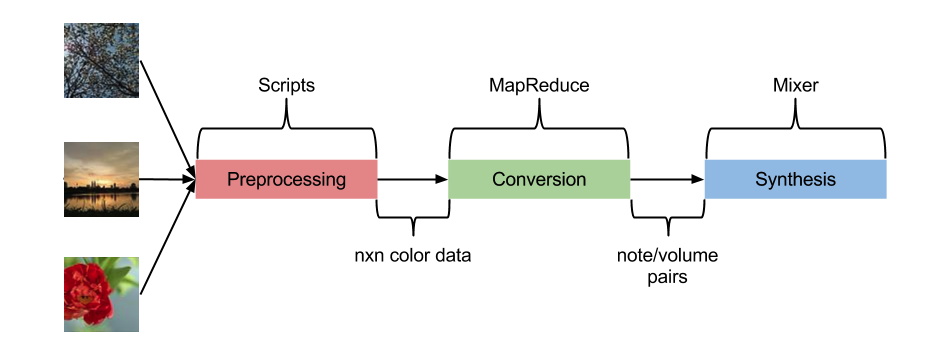
\includegraphics[width=.85\textwidth]{pipeline.png}
  \caption{High level view of the pipeline used for the project}
  \label{fig:project-pipeline}
\end{figure*}

Our implementation consists of scripts to transform the input,
MapReduce phases, and a music mixing tool.  The high level pipeline is
shown in Figure~\ref{fig:project-pipeline}.  It consists of a sequence
of MapReduce jobs, along with sets of helper scripts 

\subsection{Conversion of images to thumbnails}

Conversion to music happens by doing operations on colors and image
data.  To do the conversion to tone, velocity pairs, we transform
colors in the input data, meaning that we have to start with a
representation of $R$ colors for each image.  To do this
transformation, we considered using a MapReduce job: mapping over the
sets of images in our input corpus.  Ultimately we found that
converting images to thumbnails was better accomplished using scripts:
which allowed us to do other manipulation as well.  We anticipate that
if this became a problem we could have moved the image processing code
to Java and pass in our input corpus to the initial stage of
MapReduce.  Our current implementation uses the RMagick \cite{rmagick}
gem, which is a Ruby library interfacing to ImageMagick
\cite{imagemagick}.  ImageMagick includes facilities for taking images
to thumbnails, we simply use the RMagick library to preprocess all of
our images so that they are in the correct dimensions and are of the
proper size.

%% \begin{figure}
%% \begin{lstlisting}[language=Ruby]
%% require 'rmagick'

%% class ThumbMaker
%%   # Convert set of images to thumbnails
%%   def self.convert_thumbs(dir_path, size)
%%       # ... 
%%       puts "Making thumbnail for..."
%%       Dir.glob("#{path}/*.jpg") do |fname|
%%         # ...
%%         fname = # ...
%%         img = Magick::Image.read(fname)[0]
%%         thumb = img.thumbnail(size, size)
%%         thumb.write(thumb_dest)
%%       end
%%     end
%% end

%% \end{lstlisting}
%% \caption{Relevant code from the module used for image to thumbnail
%%   conversion}
%% \end{figure}

\subsection{Conversion to intermediate representation}
\label{sec:conversion}
Image data comes in a variety of different formats: JPEG, GIF, PNG,
etc..  Dealing with the plethora of formats presents a problem for our
translation because there are many artifacts of the formats
(annotations, geotagging, compression, etc..) which are unnecessary
for our implementation.  To keep the core abstraction of images as
arrays of bytes (the abstraction described in
Section~\ref{sec:overview}) the first stage of our Hadoop
implementation converts the surface image representation to the
sequence file format used in subsequent processing.  Although it may
appear inefficient to hold an uncompressed image in memory, this is
actually ideal for Hadoop: because computing cycles (incurred through
recompressing and sending the images) are the cost, compared with
network traffic.

The conversion in our prototype uses the java \code{ImageBuffer}
class to do image input and conversion.  This class holds requires a
large amount of memory to represent image objects, however this is
fine because we hold only a small number of images in memory at any
one time (using statics) when mapping over our input corpus.


Our implementation for this conversion happens in the
\code{WriteImagesToSequenceFile} class.  They key novelty in this
class is the conversion of image data to a \code{SequenceFile} based
representation.  A \code{SequenceFile} works well for our application
because we need to stream potentially large amounts of image data (raw
bytes).  This is fundamentally no different than creating a custom
Writable instance to serialize to a \code{SequenceFile} at a later
point, but given the simplicity of our representation we say no need
to do this.

\subsection{Translating to note, region pairs}

After taking the image data to an intermediate format, we must map the
image data to a set of note / region pairs for use in the MIDI.  To do
this, we map a conversion function across each of the different
portions of each image.  The conversion happens by mapping over our
set of images in the \code{Image2MusicMR} class.  The input of this
reducer is a set of key/value pairs which constitute the image number
and image data (a set of integers representing each pixel in the
image).  The output of the image to music conversion is $n$ sets of
note lists (where notes are expressed as pairs).  This is stored as a
set of key/value pairs where the key is the region number and image
number pair (subsequently discussed, but used for secondary sorting)
and the part number and MIDI note.

The strategy used in the conversion is to map over each pixel in an
image, apply the conversion function, and emit it to a reducer to
collate together.  After mapping over each pixel, we need to end up
with a stream of images for each region: a na\"{i}ve implementation simply
maps each pixel in our input corpus to these tone, velocity pairs:

\[
  map : id \times (r,g,b) \to region \times (tone \times velocity)
\]

However, when we actually mix the music, we need each of the streams
to be in an ordered format.  Because the default sorting order does
not take this into account, the music ends up jumbled (each of the
regions is permuted with respect to input ID in an arbitrary way).  To
fix this, we perform secondary sorting on the input ID:

\[
  map : id \times (r,g,b) \to (id \times region) \times (tone \times velocity)
\]

\subsection{Mixing and producing playable music}

The result of our mapreduce pipeline is a set of notes in MIDI: one
for each region in the image set.  We postprocess the MapReduce output
by taking it off HDFS using a script and converting to the MIDI format
(adding on a header about the number of parts and other small details
to be a valid MIDI file). To turn these into music that can be played,
we use mixing software (such as GarageBand) to mix the regions into
full scores and generate MP3 files.

To visualize music and colors, we take the resulting music and mix it
with a video generated from the thumbnailed images in our input
dataset.  We do this using a process similar to preprocessing: we
simply blow up the thumbnailed images to a larger size, concatenate
them together into subsequent frames of a video, and mix the video
with the music generated from our MapReduce phases.

\section{Results}

To test the system, we use a variety of different sets of images.
These images were obtained from
Flickr\footnote{\url{http://www.flickr.com/}} and \code{memebase.com},
using a public API and a Python script \cite{flickrpy} to get test
data.  We converted animated GIFs into individual frames again using a
preprocessing phase.  Our MapReduce code takes as input simply a
\code{SequenceFile} (as discussed in Section~\ref{sec:conversion}), so
we simply feed in a folder of JPG images to our preprocessing phase.

As a result, we produced various pieces of music.  Our longest piece
(named \code{Digital Nightmare}) was over six minutes long and
composed of over 3500 images.  We also produced shorter (self
contained) pieces from various related images: such as GIFs of cat
jumping animations.  All of these pieces are made available in our
repository.  We ran the entire MapReduce job on the Hoth cluster to
produce our longest piece.

Our MapReduce phases ran very quickly (on the order of minutes, mostly
startup time).  We believe that the reason for this is that by the
time preprocessing was completed we ended up with a relatively small
amount of data to be fed into MapReduce.  Were we to do the project
over again we would have fed in much more data to the MapReduce jobs
and optimized the selection of regions (from each image) to be the
``best sounding'' piece of music that could be produced.  We thought
about how to devise a measure of ``realistic'' music, but could not
easily see one.  One potential next application would be to use Hadoop
to mine this correlation.  The idea is that realistic music generally
has some recurring nature (backbeat, for example) even if very
complex.  Therefore, we would want to apply a penalty term to our
measure whenever we generated music that had too complex a principal
structure (this would avoid creating chaotic sounding music).  We did
some initial work on this (writing down some equations, studying how
to analyze MIDI for it's beat) but didn't have anything concrete by
the time we needed to do implementation.

We also noticed that there might be some interesting problems in
taking a song and a set of videos and finding out which best matched
each other.  (In essence, this would let you search for image based on
video.)  We started to write an inverse transformation within
MapReduce\footnote{src/main/phase2/Color2Music} to explore this idea,
but haven't finished doing the work yet.

\subsection{Reflection on Results}

One might describe our final piece, \emph{Digital Nightmare}, as an unrelenting flood of almost patternless musical information.
This characteristic emerges from some simplifications in design choices that a later vernon of our process would look to address.
Here we present a list of such areas and possible solutions.

\begin{itemize}

\item Each instrument plays a note during every musical time unit
  (beat). This results in constant note information without any space
  for the listener to "catch up".  Darker colors below some threshold
  of brightness could all be translated into musical rests.

\item Each note played last only one beat, i.e quarter notes are the
  only length note used.  Consecutive image regions with similar
  colors could be "strung together" cause some instruments to play
  longer notes.

\item Late on in the process, we moved from saturation mapping to
  velocity to choosing a fixed velocity of 127.  We found that
  velocity dynamics were not so perceptible with the degree of musical
  production we were willing to invest.  Spending more time in the
  post-processing phase and focusing on musical dynamics such as
  volume, panning, etc could improve the contribution of velocity to a
  musical piece.

\item In our final piece, saturation did not contribute to velocity,
  but instead was a component of the octave calculation. This choice
  was made after observing some short musical pieces and feeling that
  the color to sound mapping was not as intuitive as we had expected.
  This change helped somewhat, but we feel the issue was related to a
  number of factors including the limitations of the HSB color model
  to represent the human visual model, the discretization of a
  continuous range (color is continuous whereas music notes are
  discrete), and using a constant scale rather than a logarithmic
  scale to represent musical frequencies (which are inherently
  logarithmic, each an octave higher is twice the lower octave's
  frequency).

\end{itemize}

\section{Related work}

Our work is inspired by the music visualization effects included in
media player software (which traditionally includes effects such as
oscilloscopes and frequency representations).  However, many domain
specific programming languages exist for music synthesis.  In
particular we looked at Haskore \cite{haskore} and
LilyPond\cite{lilypond}.  Haskore is a language based on Haskell,
which allows the user to express mathematically beautiful music using
an algebraic composition strategy.  LilyPond is a specification
language used to create high quality sheet music (similar to \LaTeX\ 
for music).  Many of these languages synthesize music in the small,
using a human based specification language.  By contrast, our approach
focuses on using large amounts of data to create music: rather than a
human specification.  We are unaware of any projects that use big data
to produce art or other forms of entertainment.

\section{Conclusion}

At the onset of this project, we had a vision for translating images
in music and we have succeeded in doing so.  Just about every design
decision in our process has room for improvement, we are pleased to
have at least found a path from start to finish, though not without
trials.  At every stage of the pipeline, there were new complexities
to discover --- the various color models and their relationships, the
difficulty in using natural language to discuss color, or the vast
number of parameters needed for machines to represent a piece of audio
or visual art.  However challenging though, the journey has put into
perspective the amazing ability of the painter and composer to produce
works of art with far more complexity than machines can manage.  We
hope that our work inspires technologists to apply their skills to
reinterpret works of others from unrelated fields, and vice versa.

\bibliographystyle{IEEEtran}
\bibliography{paper}

\end{document}
